
\chapter{Introducción}
\label{chap:introduccion}

\drop{E}{}n el año 1943 el Dr. Abraham Maslow, uno de los fundadores y
máximo exponente  de la psicología  humanista, propuso la  <<Teoría de
las     necesidades      humanas>>~\cite{Maslow}.   Esta publicación  obtuvo una  gran notoriedad,  no
sólo en el ámbito psicológico sino  también en el empresarial debido a
que define  muy bien una jerarquía  de las necesidades humanas,  en la
que la satisfacción  de las necesidades más básicas  o subordinadas da
lugar  a   la  generación   sucesiva  de   necesidades  más   altas  o
superordinadas.  Otro principio  fundamental de  su teoría  es el  que
sugiere que las únicas necesidades que  nacen con el individuo son las
de  la base  es decir  las necesidades  fisiológicas y  que las  demás
surgen a partir de estas necesidades una vez que ya han sido suplidas.

Como podemos ver en la pirámide de Maslow (véase Figura~\ref{fig:maslow_pyramid}), la seguridad, en todo su conjunto, ocupa el segundo escalón más importante dentro de las necesidades humanas, quedando sólo por detrás de las necesidades fisiológicas.

\begin{figure}[!h]
\centering
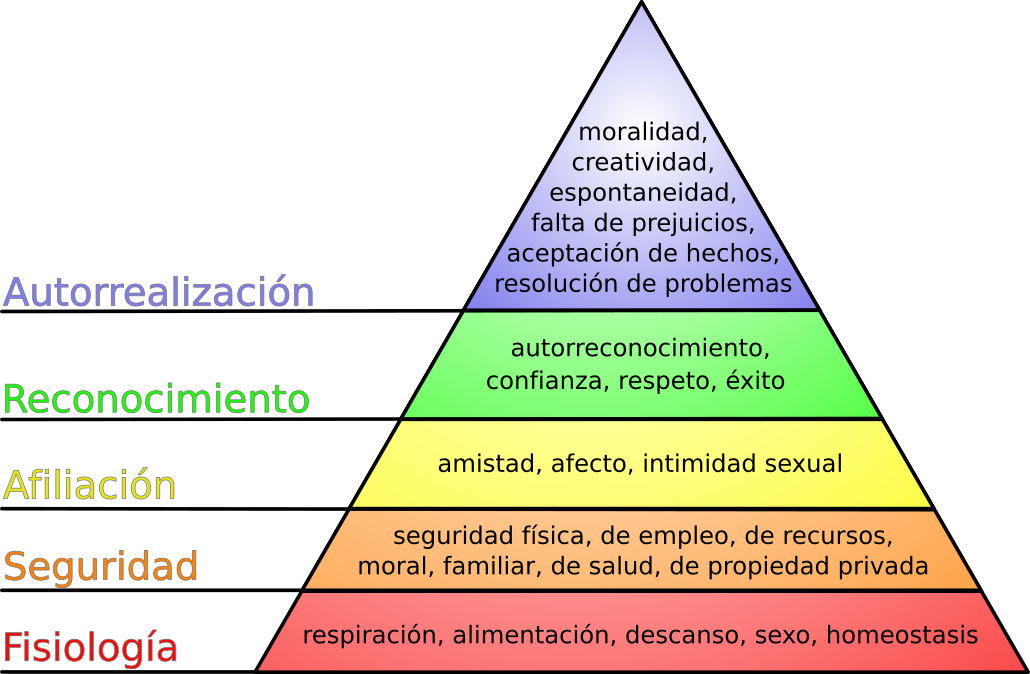
\includegraphics[width=0.8\textwidth]{/maslow_pyramid.png}
\caption{Pirámide de Maslow~\cite{Maslowpyramid}}
\label{fig:maslow_pyramid}
\end{figure}

Tomando como base lo expuesto anteriormente y la impetuosa necesidad del ser humano de sentirse seguro, en nuestro caso, físicamente, el hombre a medida que han avanzado los tiempos ha ido diseñando nuevos sistemas de seguridad que se adaptasen mejor a las nuevas posibles amenazas.

Por lo  general estos  sistemas de  seguridad no  suelen ser  un único
servicio  aislado  sino  que  se  comprenden  de  una  combinación  de
elementos físicos y electrónicos que en su conjunto dan como resultado
la herramienta adecuada  para tratar de salvaguardar  la integridad de
personas,  bienes  materiales  y   recintos,  mediante  la  colocación
estratégica de varios  dispositivos con el fin  de detectar presencias
no autorizadas e intrusiones.

Hoy  en  día, los  sistemas  de  seguridad  tienen  un alto  grado  de
automatización  basado en  un conjunto  de sensores  y tecnologías  de
comunicaciones,  así  como  software   de  gestión  que  evalúan  las
potenciales situaciones de riesgo y son capaces de reaccionar de forma
autónoma o como apoyo al personal de seguridad.

Con  el propósito  de estandarizar  algunos aspectos  relativos a  los
sistemas de seguridad  privada, en el año 2011 se  emiten una serie de
órdenes ministeriales en  las que se establece  una categorización, en
grados de  seguridad, para  las instalaciones y  los elementos  que la
conforman, atendiendo  a los niveles de  riesgo a los que  cada uno de
ellos hace frente. Así, un \acf{GII} se refiere a un nivel de riesgo bajo a medio, dedicado a viviendas y pequeños establecimientos, comercios e industrias en general, que pretendan conectarse a una central receptora de alarmas o, en su caso, a un centro de control. El \acf{GIII} queda reservado para instalaciones de riesgo medio/alto en establecimientos comerciales o industriales a los que por su actividad se les exija disponer de conexión a central receptora de alarmas o, en su caso, a un centro de control. Para esta última categoría o grado, se exige que tanto los detectores como los contactos magnéticos e infrarrojos puedan presentar los estados de: alarma, reposo, tamper, cortocircuito y sabotaje~\cite{BOE}.

Aunque hace unos años los sistemas de seguridad eran utilizados en el ámbito industrial mayoritariamente, hoy en día existen alternativas adaptadas al mercado doméstico que han provocado una rápida evolución y aparición de nuevos dispositivos, sistemas y fabricantes que operan en este sector. 

Sin embargo, tradicionalmente, el sector de la seguridad ha estado dominado prácticamente en su totalidad por tecnologías propietarias. Este tipo de sistemas constan habitualmente de una central y software de gestión que se licencian en función de las características de la instalación y en algunos casos por períodos contratados. Además, la mayoría de estos sistemas tradicionales se basan en una arquitectura centralizada, siendo más vulnerables ante fallos, tanto arbitrarios como intencionados, ya que tienen un punto de fallo central que inutiliza todo el sistema. 

Por otra parte,  el grado de penetración de las  nuevas tecnologías de
cara a la  usabilidad de las interfaces de usuarios  es escasa en este
sector. La gran  mayoría de aplicaciones de  gestión poseen interfaces
poco  amigables e  intuitivas que  dificultan  su uso  a usuarios  sin
formación  previa, haciendo  que en  ocasiones  no se  exploten en  su
totalidad las funcionalidades que realmente brindan los sistemas.

Esta situación ha provocado que el mercado adopte como norma este método de trabajo, dificultando seriamente la entrada de nuevos productos salvo para aquellas empresas que ya disponen de renombre o que poseen un capital considerable como para hacerse un hueco en la industria de la seguridad~\cite{garc2007hesperia}.

Teniendo en cuenta todo lo anterior y atendiendo al panorama actual de los sistemas de seguridad privada, se puede afirmar que los avances tecnológicos no están siendo apropiadamente adoptados por esta industria~\cite{PPavan2015}. En este sentido, la aparición de plataformas hardware de bajo coste como Arduino\footnote{\url{https://www.arduino.cc/}} y las oportunidades que se derivan de su capacidad de interconexión plantean un escenario idóneo para estudiar su posible aplicación a entornos tan restrictivos como el de la seguridad.  

\begin{figure}[!h]
\centering
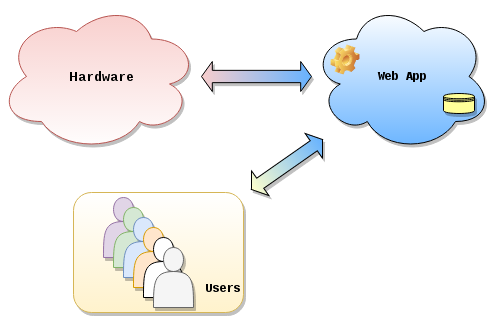
\includegraphics[width=0.8\textwidth]{/basic_system.png}
\caption{Diagrama de Sistema de Seguridad Oshozi}
\label{fig:basic_system}
\end{figure}

Por todo ello,  en este \acf{TFG} se pretende  abordar estos problemas
desarrollando un sistema completo de seguridad, utilizando hardware de
bajo  coste.  El  enfoque  principal de  esta  solución  será  ofrecer
interoperabilidad,   de   modo   que   dispositivos   de   fabricantes
cualesquiera, puedan coexistir para  realizar despliegues no triviales
(véase  Figura~\ref{fig:basic_system}).  Para  lograrlo,  es  esencial
utilizar  protocolos  y  mecanismos   de  interacción  abiertos,  bien
documentados y reconocidos por la comunidad, igual que ocurre en otros
muchos  ecosistemas como  pueden ser  la telefonía  móvil. Además,  se
pretende abordar la problemática de la centralización, proponiendo una
arquitectura  más  descentralizada  en  la que,  ante  fallos  en  las
comunicaciones o  en los  sistemas de gestión,  se pudiera  ofrecer un
comportamiento  degradado,  de  modo  que  controladores  individuales
puedan seguir ofreciendo valor a la instalación.


No obstante a todo lo expuesto aquí, actualmente hay fabricantes que se esfuerzan no sólo por llegar a satisfacer las necesidades del mercado, sino también por innovar. Un ejemplo de plataformas integradoras puramente españolas son: Desico\footnote{\url{http://www.desico.com/es/}} y Dorlet\footnote{\url{http://www.dorlet.com/}}. Ambas empresas venden sistemas o plataformas de integración donde ofrecen gestión de los elementos de intrusión, CCTV, control de accesos e interfonía sobre la misma interfaz, pero en ambos casos y por lo costoso de las certificación en grado, no ofrecen su producto como un sistema de seguridad como podría ser Honeywell~\cite{Honeywell}, que fabrica principalmente centrales de seguridad de \acs{GII} y \acs{GIII}.


\section{Estructura del documento}

A continuación se expone la estructura del documento y una breve reseña del alcance de cada una de las partes.
\begin{definitionlist}

\item[Capítulo \ref{chap:objetivos}: \nameref{chap:objetivos}] Donde se enuncia el objetivo general que se busca y se concretan los objetivos específicos marcados para conseguirlo.
\item[Capítulo \ref{chap:antecedentes}: \nameref{chap:antecedentes}] Donde se exponen los conocimientos elementales para comprender el resto del documento. Se describen algunos de los principales sistemas de seguridad que compiten en el mercado y la visión de los fabricantes sobre la evolución del mismo.
\item[Capítulo \ref{chap:metodologia}: \nameref{chap:metodologia}] Donde se describe y se expone el porqué de la metodología elegida para el desarrollo del proyecto, los pasos seguidos y en que han consistido desde el punto de vista metodológico.
\item[Capítulo \ref{chap:desarrollo}: \nameref{chap:desarrollo}] Donde se describe la arquitectura del sistema desarrollado y se exponen las consideraciones de diseño más importantes.
\item[Capítulo \ref{chap:conclusiones}: \nameref{chap:conclusiones}] Donde se exponen las conclusiones generales obtenidas del trabajo realizado abordando la consecución de los objetivos propuestos y se plantean trabajos futuros.
\end{definitionlist}
